\begin{landscape}
\begin{figure}
    \centering
    
	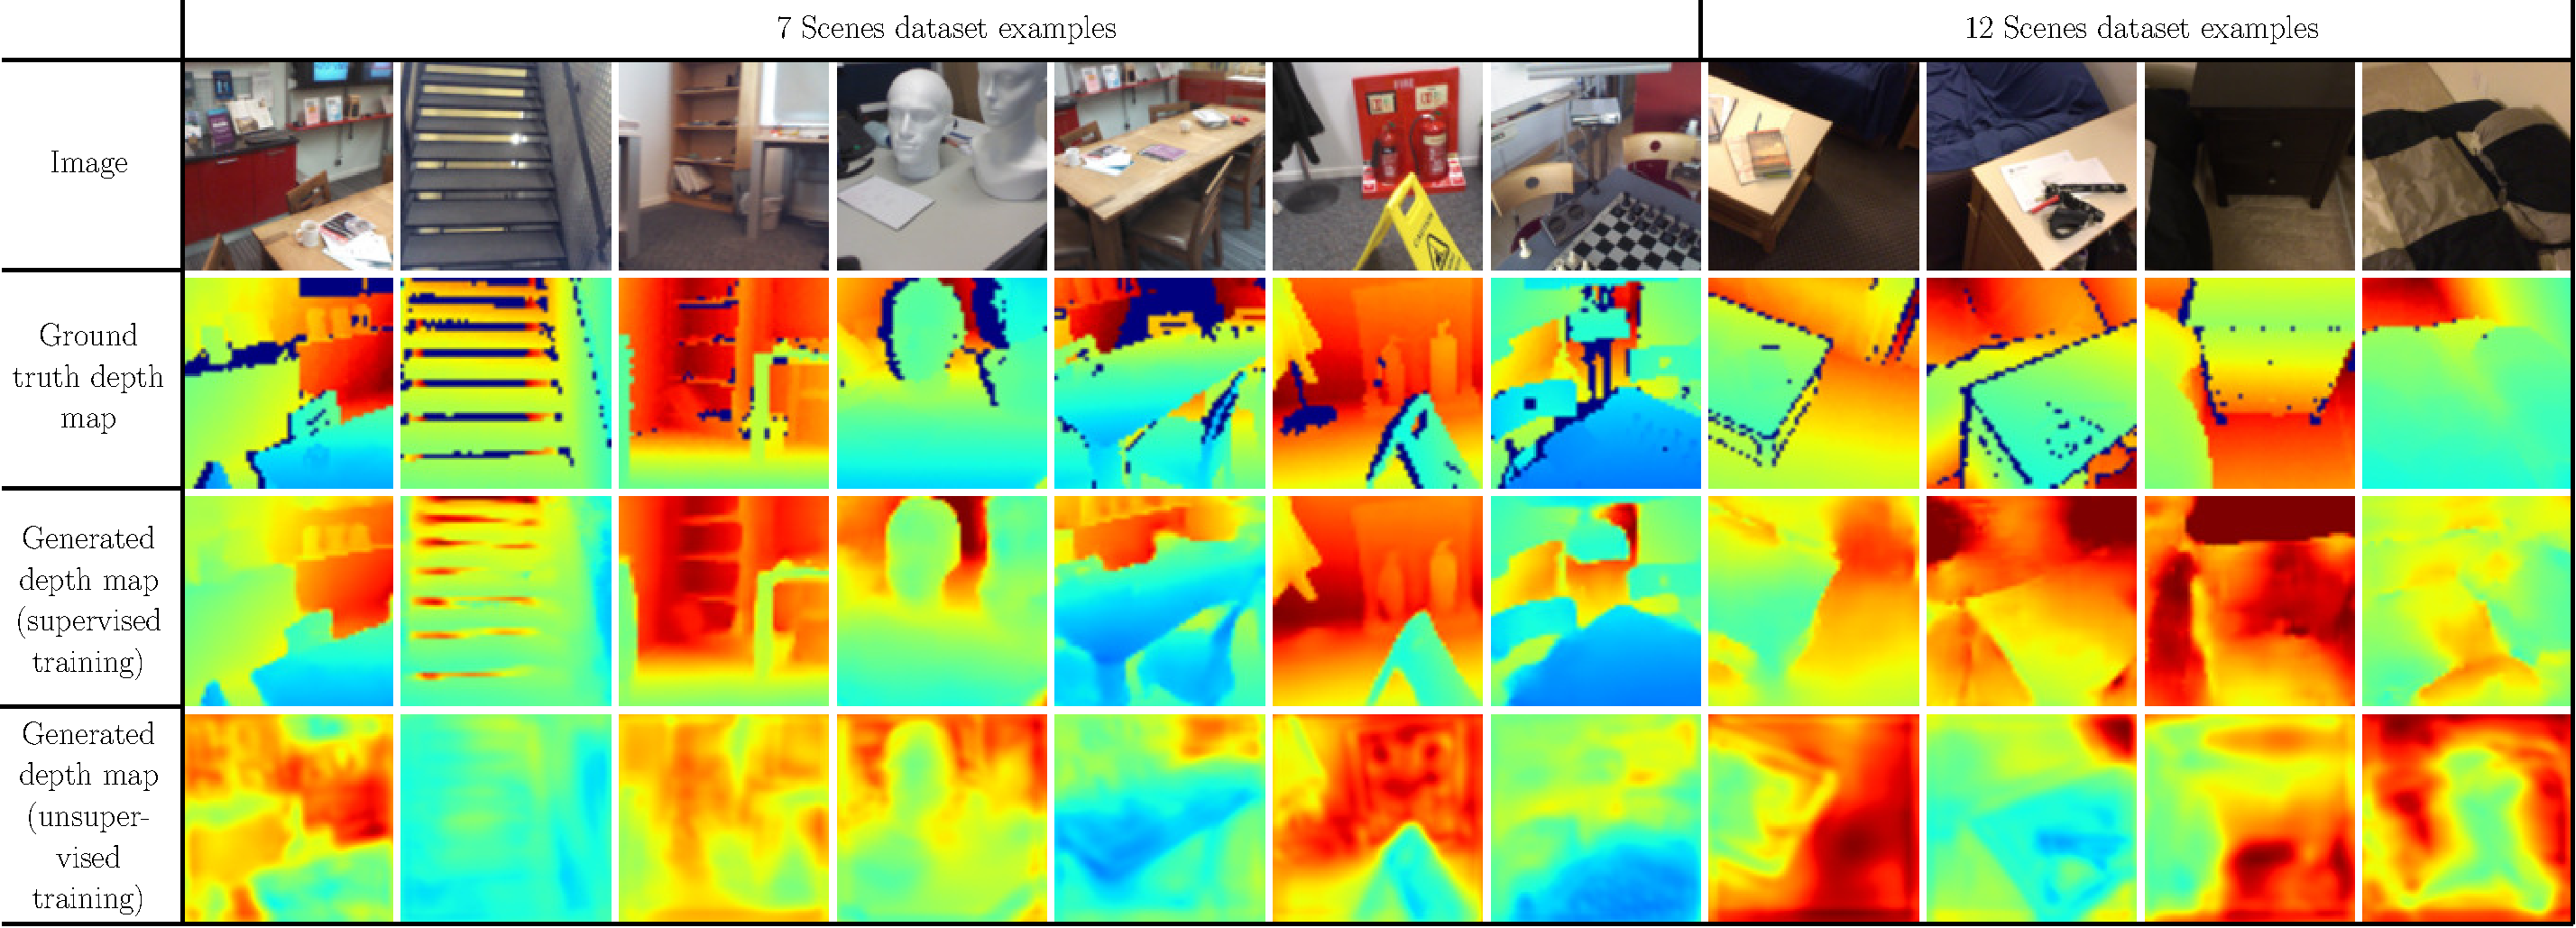
\includegraphics[trim={96 0 0 0},clip,width=\linewidth]{results/indoor/depth_maps}
	\caption[Generated indoor depth maps]{\label{fig:depth_map_indoor} \textbf{Visualization of the depth map generated from RGB input:} from top to bottom: image, ground truth depth map, generated depth map (supervised training), generated depth map (unsupervised training). In both configurations (supervised and unsupervised), networks are trained on the \textbf{7 scenes} dataset~\citep{Shotton2013}. Examples from \textbf{12 scenes}~\citep{Valentin2016} show networks generalization capability.}

\end{figure}
\end{landscape}
